\subsection{Extension to Other Error Models}
In many cases {FLE} cannot be properly modelled as an isotropic, independent, random variable. In the case of optical tracking systems for example \cite{736031} the errors normal to the camera plane are approximately 3 times those parallel to the camera plane. It is straightforward to implement such an anisotropic \gls{FLE} in SciKit-SurgeryFRED and test the effect on registration outcomes.

The following code snippet is taken from  main.py. Line 63 defines the ratio of \gls{FLE} in three directions. By default they are all equal.

\begin{lstlisting}[language=python, firstnumber = 54]
@app.route('/getfle', methods=['POST'])
def getfle():
    """
    Returns values for fiducial localisation errors
    Values are randomly selected from a uniform
    distribution from 0.5 to 5.0 pixels
    """
    fle_sd = np.random.uniform(low=0.5, high=5.0)
    #change fle_ratio if you want anisotropic fle
    fle_ratio = np.array([1.0, 1.0, 1.0], dtype=np.float64)
    anis_scale = math.sqrt(3.0 / (np.linalg.norm(fle_ratio) ** 2))
    fixed_fle = fle_ratio * fle_sd * anis_scale

    moving_fle = np.array([0., 0., 0.], dtype=np.float64)
    fixed_fle_eavs = expected_absolute_value(fixed_fle)
    moving_fle_eavs = expected_absolute_value(moving_fle)

    returnjson = jsonify({
            'fixed_fle_sd': fixed_fle.tolist(),
            'moving_fle_sd': moving_fle.tolist(),
            'fixed_fle_eav': fixed_fle_eavs.tolist(),
            'moving_fle_eav': moving_fle_eavs.tolist()
            })
    return returnjson
\end{lstlisting}

Changing line 63 to;
\begin{lstlisting}[language=python, firstnumber=63]
    fle_ratio = np.array([3.0, 1.0, 1.0], dtype=np.float64)
\end{lstlisting}
sets the error in the x direction to 3 times that in the y and z directions. The results of this modification are shown in Fig. \ref{fig:anis_error}. 

\begin{figure}
	\begin{center}
		\begin{subfigure}[b]{0.48\linewidth}
			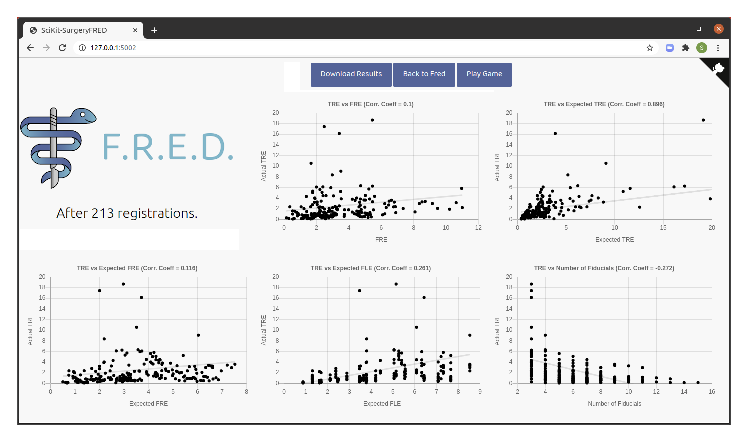
\includegraphics[width=\linewidth]{images/anisitropic_error.eps}
			\caption{\label{fig:anis_error}Anisotropic Errors}
		\end{subfigure}
		\begin{subfigure}[b]{0.48\linewidth}
			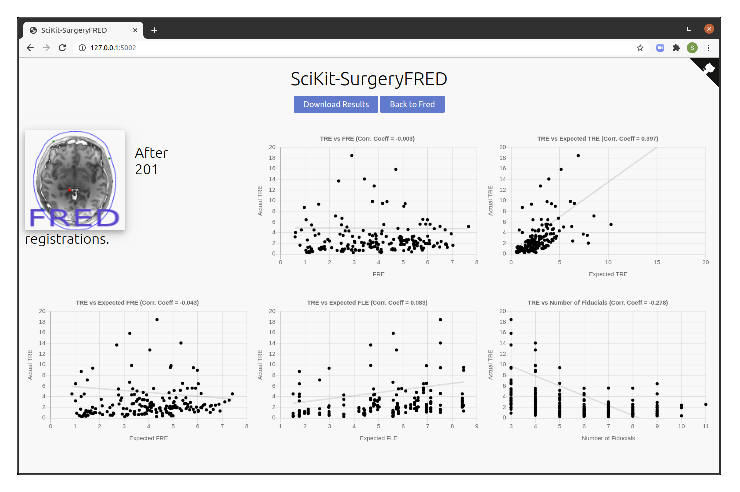
\includegraphics[width=\linewidth]{images/systematic_error.eps}
			\caption{\label{fig:sys_error}With Systematic Errors}
		\end{subfigure}
		\caption{\label{fig:other_errors}Results of over 200 registrations using an anisotropic model of {FLE} and a model with systematic {FLE}.}
	\end{center}
\end{figure}

A second significant source of error that is usually overlooked is the presence of systematic errors. For example when using a tracked pointer for fiducial localisation, 
any pointer calibration error will be be added to all fiducial markers.
Similarly some optical tracking systems can introduce a systematic error on 
the tracking markers \cite{6294449}. {SciKit-SurgeryFRED} allows systematic error to 
be added to each fiducial. The fiducial localisation error is set within 
the JavaScript function init{\textunderscore}fles()
(defined in static/main.js) each time a new target is set. 
\begin{lstlisting}[language=java, firstnumber = 429]
/**
 * Sets the global fiducial localisation error (FLE)
 */
function init_fles() {
  fetch("/getfle", {
      method: "POST",
    })
    .then(resp => {
      if (resp.ok)
        resp.json().then(data => {

        let preOpFLEStdDev = data.moving_fle_sd;
        let intraOpFLEStdDev = data.fixed_fle_sd;
        let preOpFLEEAV = data.moving_fle_eav;
        let intraOpFLEEAV = data.fixed_fle_eav;

        let preOpSysError = [0.0, 0.0, 0.0];
        let intraOpSysError = [0.0, 0.0, 0.0];

        FLE = { preOpFLEStdDev, intraOpFLEStdDev,
                preOpFLEEAV, intraOpFLEEAV,
                preOpSysError, intraOpSysError };

      });
    })
    .catch(err => {
      console.log("An error occured setting fles", err.message);
    });
}
\end{lstlisting}
By default there is no systematic error, (lines 445 and 446). We can 
add a systematic interoperative error at line 446 as; 

\begin{lstlisting}[language=java, firstnumber = 446]
        intraOpSysError = [1.0 * (Math.random()-0.5), 
                           1.0 * (Math.random()-0.5), 
                           1.0 * (Math.random()-0.5)];
\end{lstlisting}

In this case the error is an isotropic uniform random variable, in the range
-0.5 to 0.5. This error will be applied to all fiducial markers for a 
given registration. The results of this modification are shown in Fig. \ref{fig:sys_error}.

